
\subsection{Virtual Closed-Loop Prosthesis}
 \begin{figure*}[h]
		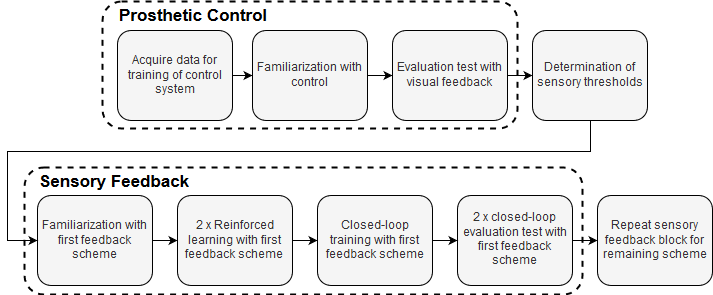
\includegraphics[width=.85\textwidth]{figures/std_paper}
	\caption{Pipeline showing the stages of the experiment. The stages in the first block focused on developing a prosthetic control system, and evaluating the subjects' ability to control the prosthesis. Then electrotactile sensory thresholds were determined. The second block focused on training the understanding of the feedback schemes and evaluating their use in combination with prosthetic control. The sensory feedback block was repeated for the remaining feedback scheme.}
	\label{fig:pa:std_pap} 
\end{figure*}
Investigating the usability of the two sensory configurations in a closed-loop scenario required these to be interfaced with a prosthetic device, which accommodated the actuation of rotational and hand aperture DoF's. However, using an actual prosthesis might result in auditory feedback being provided to the subject through prosthetic actuation sounds, eliminating the interest of solely exploring the impact of tactile feedback. Hence, it was chosen to simulate a velocity-based virtual prosthesis which enabled evaluation of the developed feedback schemes. In figure \ref{fig:pa:gridmap} is a depiction of a grid system, where the axes corresponded to the rotation angles and hand aperture. The grid squares represented the discrete intervals that were communicated through the feedback, where the cursor was the current angle and hand aperture. 
\begin{figure}[H]                 
	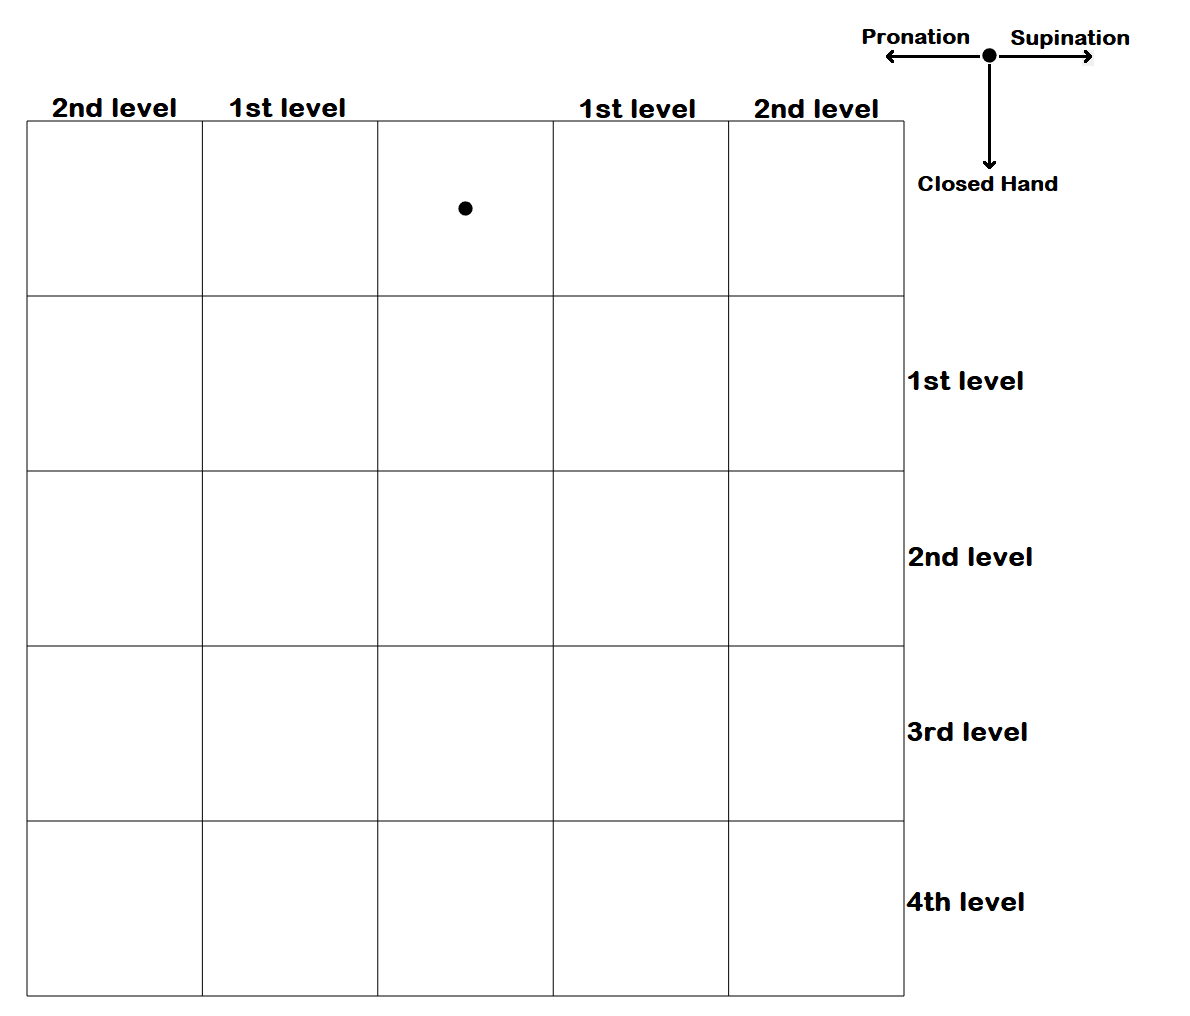
\includegraphics[width=1\textwidth]{figures/gridmap2}  
	\caption{Image of the grid map and cursor used in the experiment. Wrist supination moved the cursor to the right, pronation moved it to the left and closing the hand moved it downwards. For left-handed subjects, the rotational movements were reversed. Opening the hand moved the cursor upwards, and was used as a correction movement if needed.}
	\label{fig:pa:gridmap} 
\end{figure}

Performing supination would make the cursor move to the right and to the left when performing pronation. Performing closed hand would make the cursor move downwards and upwards when performing open hand, resembling the change in hand aperture. Performing rest (relaxing the arm) would make the cursor stand still. Furthermore, the contraction intensity was made proportional with the actuation speed, enabling the subject to have greater control of cursor movement speed. The control was sequential which only enabled the cursor to move in one DoF at a time. The control scheme thereby resembles what is typically used in commercial prostheses \cite{Atzori2015}. When the cursor entered a square a specific electrotactile stimulation would be provided corresponding to the stimulation pattern for each scheme. In the neutral position (location of cursor in figure \ref{fig:pa:gridmap}), no tactile feedback was provided.     

